\nTitle{Analyse multicritère}

Des deux parties précédentes, émergent 8 propositions de gestion de l'atelier.
Le but de cette partie sera de sélectionner la meilleure solution en fonction des 4 critères préselectionnées.

Ces 4 critères sont :
g1 : bénéfice
g2 : équilibre commercial
g3 : production
g4 : gestion du stock

\section{Méthode choisie}

La méthode de résolution choisie sera Électre \rmnum{3} car elle englobe les 2 précédentes.
On pourras ainsi fournir au client la méthode sélectionné comme la plus optimale ainsi qu'une ou plusieurs méthodes alternatives.

Pour réduire au maximum l'échéance, nous avons parallélisé au maximum les flux de travail.
Nous avons donc dès le début du projet commencé à coder sous Matlab un
algorithme de résolution de Électre \rmnum{3} indépendamment des résultats des 2 premières parties.

\section{Algorithme de la méthode}

TODO

\section{Mise en œuvre de la méthode}
L'algorithme suivant implémente la méthode Électre \rmnum{3}. À partir de la matrice des jugements, il remet à l'échelle les notes des critères en fonction des poids.

\addCode{../SourcesMatlab/electreSnippet1.m}{matlab}

Puis il calcule les matrices de concordance et de discordance.

\addCode{../SourcesMatlab/electreSnippet2.m}{matlab}


Pour finir, il établit la matrice des surclassement en fonction de ces deux dernières matrices.

\addCode{../SourcesMatlab/electreSnippet3.m}{matlab}

Un graphe est ensuite généré à partir de cette matrice, pour faciliter la lecture.
La meilleur solution apparait alors clairement en tête du graphe, et grâce à la méthode du classement et du classement inverse, on peut obtenir l'ordre des solutions.

\section{Solution proposée}

Dans un premier temps, sans pondérer les critères, on trie les solutions pour en tirer la plus avantageuse.
Après quelques tâtonnement, on utilise les seuils de concordance 0,7 et 0,9, et le seuil de discordance 0,4 pour générer un graphe de surclassement le plus clair possible, sans liens superflus.

\begin{figure}[!ht]
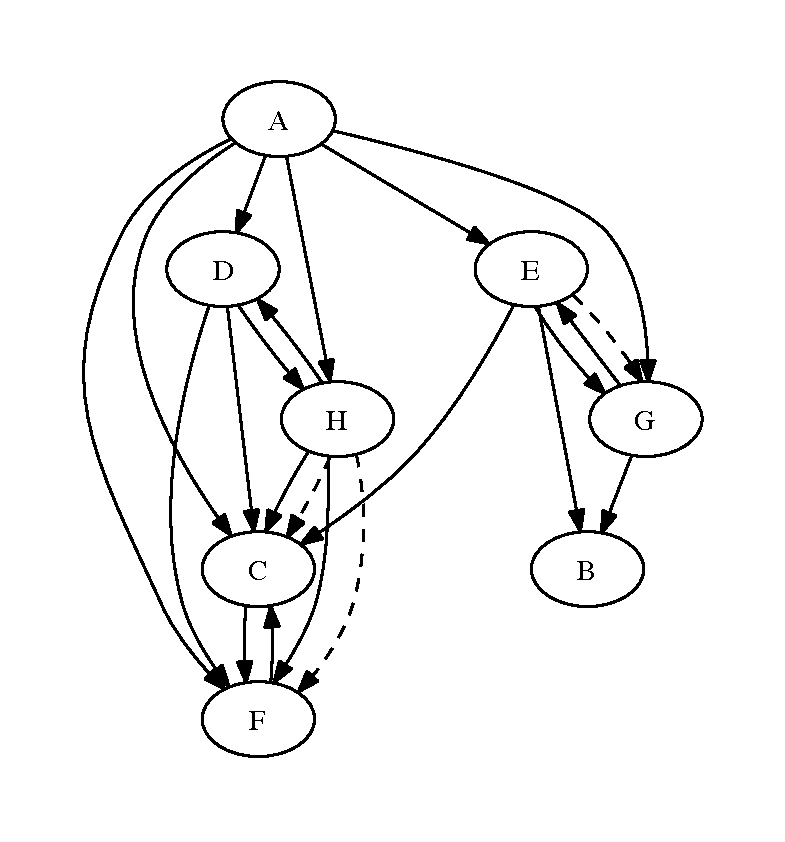
\includegraphics{../SourcesMatlab/electre3-1.pdf}
\caption{Graphe des surclassement sans prise en compte des poids de chaque critère}
\end{figure}

Sur le graphe généré, on voit clairement que la la meilleur solution serait la
solution A car c'est la seule qui n'est dominé par aucune autre.
On voit également que certaines solutions sont équivalentes puisqu'elles se
dominent entres elles. Les couples de solutions \{D, H\}, \{E, G\} et \{C, F\}
sont des couples de solutions équivalentes..
Les solutions F, C et B sont dominés, elles sont donc les moins intéressantes.


Dans un second temps, en prenant en compte les poids apporté par l'étude des 2 première parties.
